% Document Class
\documentclass[botnum, fleqn]{unmeethesis}


% Packages
\usepackage[dvipsnames]{xcolor}
\usepackage{listings}
\usepackage{rotating}
\usepackage{keyval}
\usepackage{fancyvrb}
\usepackage{xcolor}
\usepackage{float}
\usepackage{subcaption}
\restylefloat{figure}
\usepackage{ifthen}
\usepackage{calc}
\usepackage{ifplatform}
\usepackage{color}
\usepackage{rotating}
\usepackage[hidelinks]{hyperref}
\usepackage{algorithmic}
\usepackage[T1]{fontenc}
\usepackage{beramono}
% \usepackage[usenames,dvipsnames]{xcolor}



% Definitions
\definecolor{white}{rgb}{1.0,1.0,1.0}
\definecolor{lightgray}{rgb}{.9,.9,.9}
\definecolor{darkgray}{rgb}{.4,.4,.4}
\definecolor{darkcerulean}{rgb}{0.03, 0.27, 0.49}
\definecolor{purple}{rgb}{0.65, 0.12, 0.82}
\definecolor{darkred}{rgb}{0.55, 0.0, 0.0}

\lstloadlanguages{Ruby}
\lstset{
basicstyle=\ttfamily\color{black},
commentstyle = \ttfamily\color{red},
keywordstyle=\ttfamily\color{blue},
stringstyle=\color{orange}}


\lstdefinelanguage{JavaScript}{
  keywords={break, case, catch, continue, debugger, default, delete, do, else, false, finally, for, function, if, in, instanceof, new, null, return, switch, this, throw, true, try, typeof, var, void, while, with},
  morecomment=[l]{//},
  morecomment=[s]{/*}{*/},
  morestring=[b]',
  morestring=[b]",
  ndkeywords={class, export, boolean, throw, implements, import, this},
  keywordstyle=\color{blue}\bfseries,
  ndkeywordstyle=\color{darkgray}\bfseries,
  identifierstyle=\color{black},
  commentstyle=\color{purple}\ttfamily,
  stringstyle=\color{red}\ttfamily,
  sensitive=true
}

\lstset{
   language=JavaScript,
   backgroundcolor=\color{lightgray},
   extendedchars=true,
   basicstyle=\footnotesize\ttfamily,
   showstringspaces=false,
   showspaces=false,
   numbers=left,
   numberstyle=\footnotesize,
   numbersep=9pt,
   tabsize=2,
   breaklines=true,
   showtabs=false,
   captionpos=b
}

\lstdefinelanguage{JSON}{
  keywords={true, false, null},
  morestring=[b]",
  keywordstyle=\color{darkred}\bfseries,
  stringstyle=\color{darkcerulean}\ttfamily,
  sensitive=true
}

\lstset{
   language=JSON,
   backgroundcolor=\color{lightgray},
   extendedchars=true,
   basicstyle=\footnotesize\ttfamily,
   showstringspaces=false,
   showspaces=false,
   numbers=left,
   numberstyle=\footnotesize,
   numbersep=9pt,
   tabsize=2,
   breaklines=true,
   showtabs=false,
   captionpos=b
}

\lstdefinelanguage{Julia}%
  {morekeywords={abstract,break,case,catch,const,continue,do,else,elseif,%
      end,export,false,for,function,immutable,import,importall,if,in,%
      macro,module,otherwise,quote,return,switch,true,try,type,typealias,%
      using,while},%
   sensitive=true,%
   alsoother={$},%
   morecomment=[l]\#,%
   morecomment=[n]{\#=}{=\#},%
   morestring=[s]{"}{"},%
   morestring=[m]{'}{'},%
}[keywords,comments,strings]%

\lstset{%
    language         = Julia,
    backgroundcolor=\color{white},
    basicstyle       = \ttfamily,
    keywordstyle     = \bfseries\color{blue},
    stringstyle      = \color{magenta},
    commentstyle     = \color{ForestGreen},
    showstringspaces = false,
}

% Begin Document
\begin{document}

% Frontmatter
\frontmatter

\title{Student Flow Simulation with Applications in Curricular Analytics}
\author{Michael Hickman}
\degreesubject{M.S., Computer Engineering}
\degree{Master of Science\\Computer Engineering}
\documenttype{Thesis}
\previousdegrees{B.S., University of New Mexico 2014}
\date{September, \thisyear}

\maketitle
\makecopyright


% Dedication
\begin{dedication}
  Dedication goes here.
\end{dedication}


% Acknowledgements
\begin{acknowledgments}
  \vspace{1.1in}
  I would like to thank ...
\end{acknowledgments}


% Abstract
\maketitleabstract

\begin{abstract}
  Abstract goes here
  \clearpage
\end{abstract}


% ToC and Figures
\tableofcontents
\listoffigures


% Glossary
\chapter{Glossary}
Discrete-Event Simulation
JSON
\mainmatter


\chapter{Introduction}


\chapter{Background}


\chapter{Previous Work}


\chapter{Student Flow Simulation Design}

\section{Discrete Event Simulations}
Students moving through a curriculum can be viewed as a fixed, chronological sequence of events. Students will enter the university, enroll in classes, complete or withdraw from classes, then graduate if all requirements have been met. This process repeats every semester. Discrete-event simulation models a system by emulating a sequence of events, where every event occurs independently of the others at a particular instance in time and are characterized by having the following components:

\begin{itemize}
\item \textbf{Starting and Ending States} - The simulation will begin in a given state and will continue until it reaches another state that represents some pre-defined ending-condition or a point in time.
\item \textbf{Clock} - The simulation must keep track of the time that has ellapsed after it begins in any time unit relevant to the domain of the simulation. The clock does not run continuously as events occur instantaneously, but it does jump to certain times as events occur.
\item \textbf{List of Events} - The system maintains a list of events that can occur during the simulation. These events are placed in a que and are usually executed based on simulation time rather than the time they were queued.
\item \textbf{Statistics} - As the ending state is not the only result of interest when running simulations, the system keeps track of various statitics based on the events that have occured.
\end{itemize}

Using these components, a simulation is constructed using the basic following logic:

\begin{algorithmic}[1]
\STATE Initialize the system
\STATE Initialize the system clock
\STATE Schedule the initial event
\WHILE{ending condition is false} 
  \STATE{Increment clock}
  \STATE{Perform next event}
  \STATE{Update system statistics}
\ENDWHILE
\STATE Output simulation results
\end{algorithmic}

Given these characteristics and basic logic flow, this type of simulation lends itself well to the process of students flowing through a curriculum within an instituion, much more so than continuous-time simulations and other analytical models; therefore, the student-flow simulation is modeled as a discrete-event simulation.

\section{Defining A Curricula}
A curriculum is the backbone of the simulation. As the goal of the simulation is to model students moving through a curriculum, the events of the simulation depend on the curriculum that is being simulated; therefore it is important to understand how they are defined. In order for a student to obtain a degree within a given academic program, a set of requirements must be met. The requirements, in most cases, are simply courses that must be passed. However a curriculum is more than a set of courses, but rather an arragement of courses with constraints as to when they can be taken. This arrangement begins by placing courses within terms where, ideally, student would take and pass the entire set of courses in one semester. Next, relationships are created between courses in the form of prerequisite and corequisite relationships. This structure of courses grouped in terms with defined relationships make up a curriculum. A visual, graph representation of a curriculum can be seen in Figure \ref{fig:curriculum_example}.

\begin{figure}[h!]
\centerline{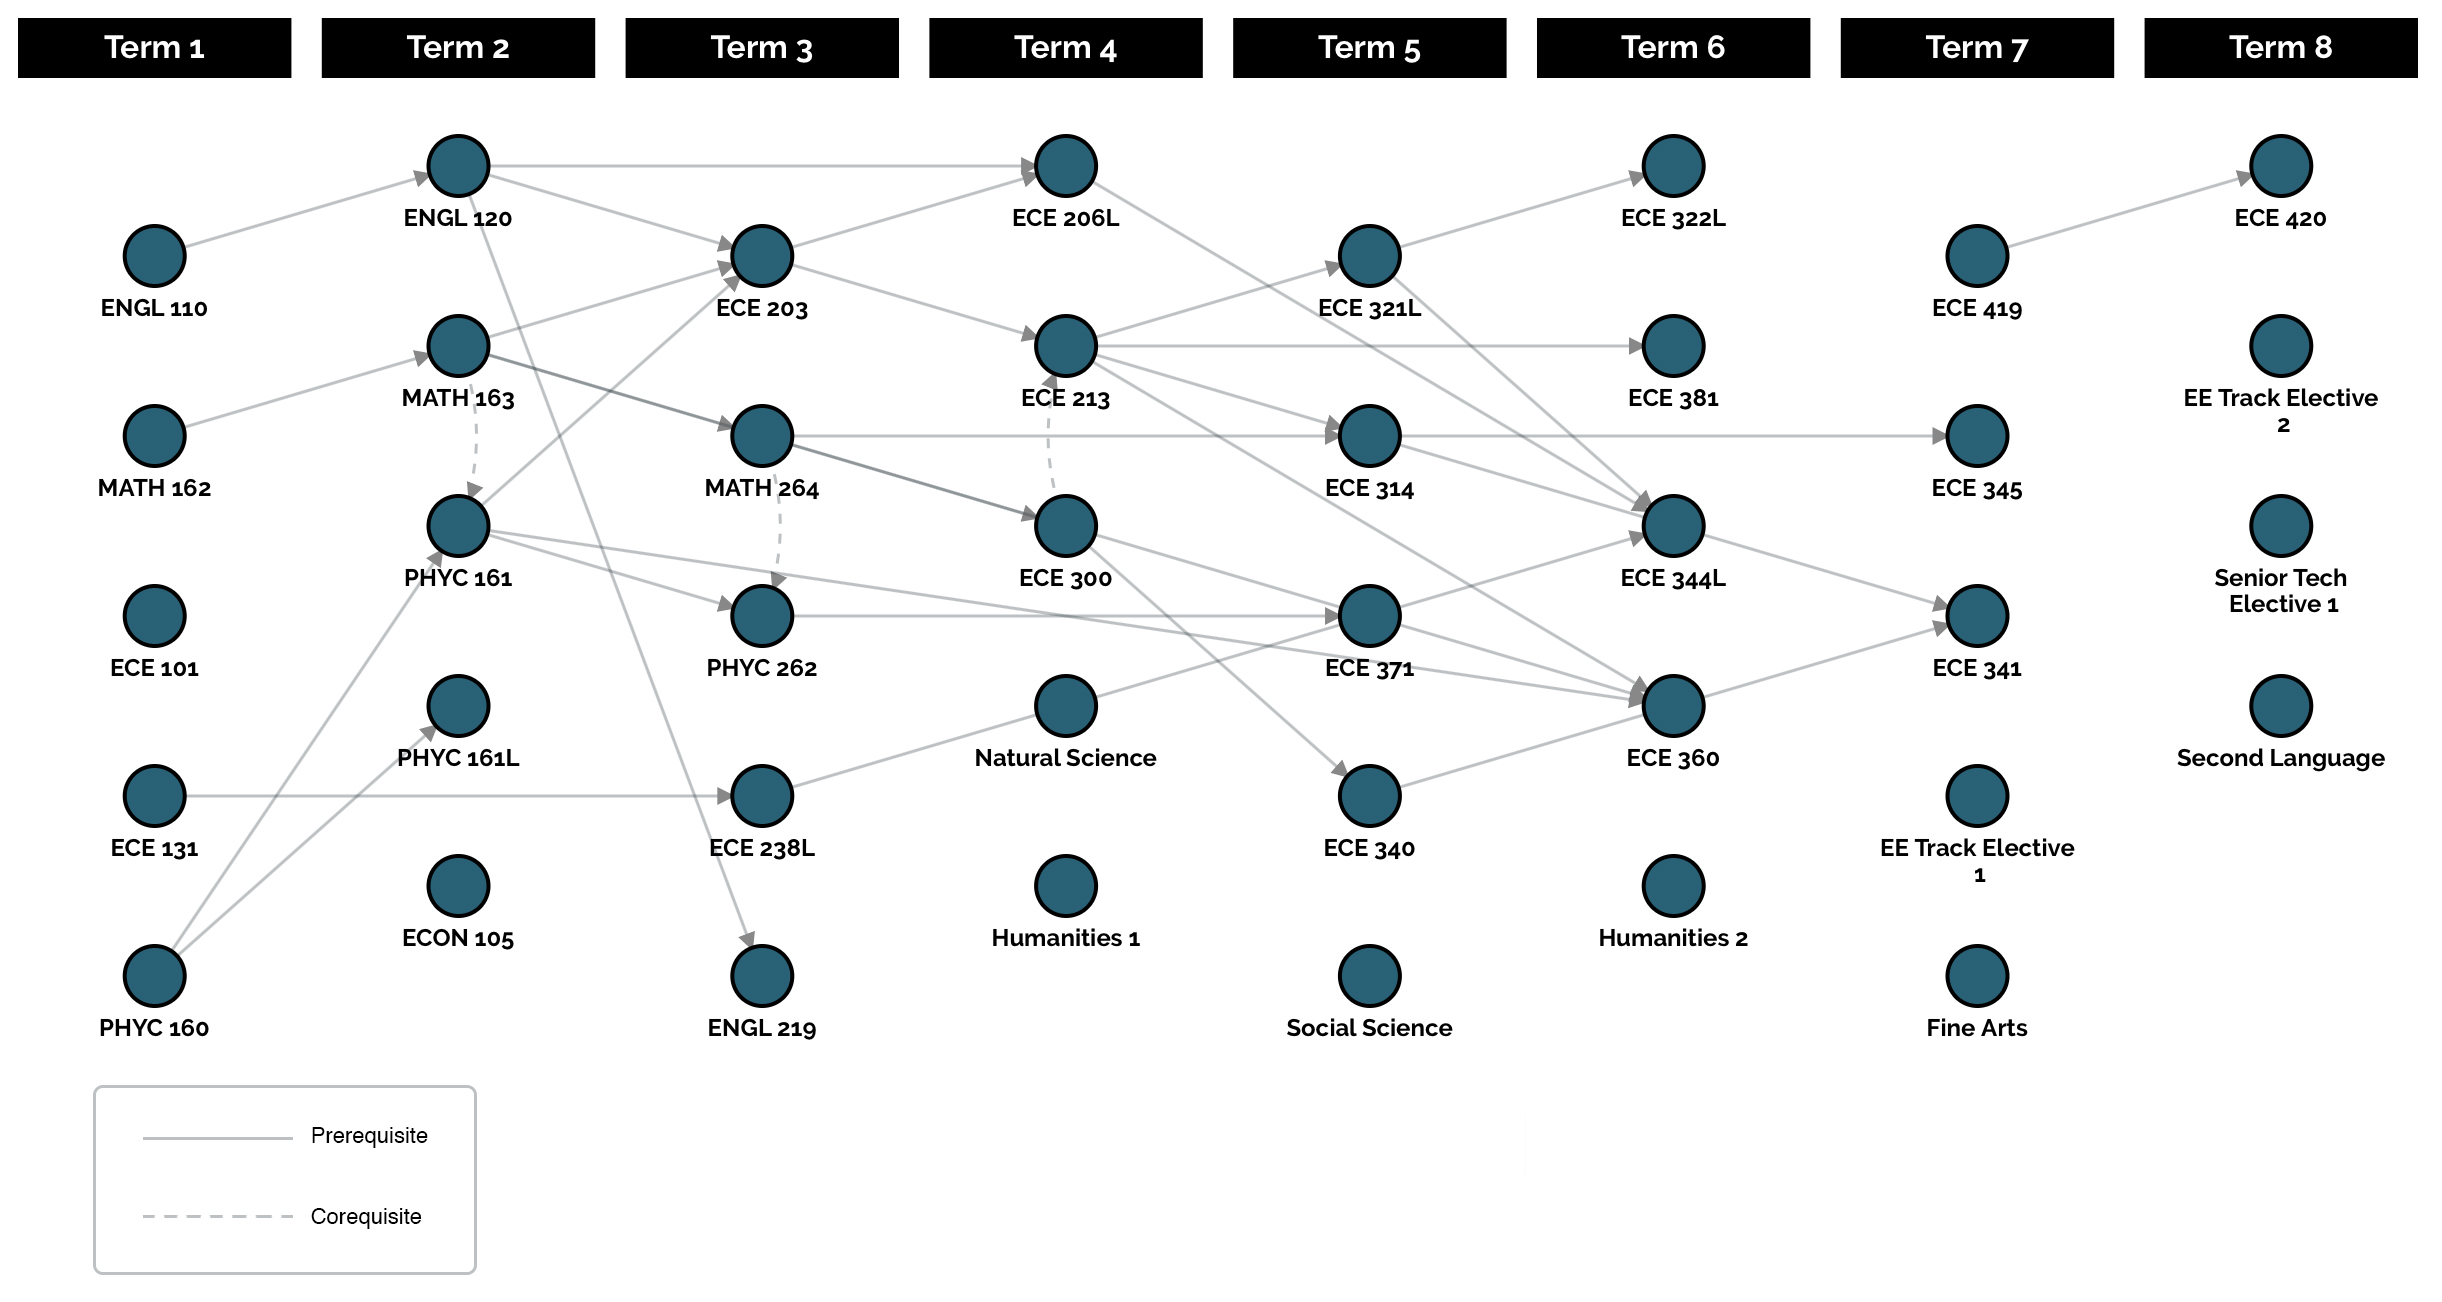
\includegraphics[scale=0.4]{./figures/curriculum_example.jpg}}
\caption{Visual representation of the electrical engineering curriculum at UNM.} 
\label{fig:curriculum_example}
\end{figure}


\section{Assumptions}
A student's academic career within an institution can potentially be a very difficult thing to model. This is primarily because student behavior can be eratic and unpredictable even given a structured curriculum. Students might not register for the courses they should, take courses that don't count, drop classes, take a semester off, get an override to take a course that they normally wouldnt have been able to, and various other actions that would otherwise not be considered \'typical' behavior. There are a vast amount of factors that can influence student behavior, many of which are not academic and would therefore be very difficult to account for. Furthermore universities can impose various policies that would also have an effect on how students register for classes and affect other academic decisions. 

Trying to realistically simulate all possible actions that a student can take would be impossible, therefore several assumptions and decisions are made to simplify student behavior down to the basics, making meaningful simulation feasible without needless complexity. The most influential decions made, was to design the student flow simulation with the primary goal of performing analytics over curricula and observing the effects their properities have on students moving through it. This is in contrast to developing a system to provide realistic simulations of student behavior with the goal of predicting graduation rates and other statistics. The simulation is potentially capable of this; however it was not the goal. Thus the other decisions made were done so to put emphasis on how curricula influence outcomes relative to one another instead of how student behavior does so. Below is a list of the other assumptions and decsions:

\begin{itemize}
  \item All students at the beginning of the simulation are treated as first-time, full-time students. Although in many cases actual freshman might have some college credit, either through AP-tests, taking college-classes while in high-school, or transfers, students in the simulation begin with a clean slate. They are also treated as fullt-time students with no notion of \'part-time' built in.
  \item Given that all students are full-time, each semester all students will register for as many credits as they can. In reality, most students do not hit their institutions max credit-hour limit, but the simulation will register students in as many courses as they are allowed - which is set by the user.
  \item The simulation only deals with a single class of admitted students. There is no continuous influx of freshman or transfer students each semester within the simulation.
  \item Students who stop-out are disenrolled permantly. They do not re-enroll.
  \item Students will only register for courses within the specified curriculum. The simulation is only aware of the courses specificied in the curriculum, so while it is common for students to register for courses that might not count towards their major, this behavior is not part of the simulation.
  \item The order of courses in which students enroll in depends on their ordering within the curriculum. Students will enroll is the earliest listed course within the curriculum and will roll in each course they can as until they hit the credit-hour limit. This process is described in greater detail later.
  \item The minimum passing grade is universal amoung all courses. This grade can be set by the user, and defaults to a C-.
  \item All course enrollment requirements are strictly enforced. While it is common for students to obtain permission and subsequent overrides to enroll in a class they have not met the requirements for, the system does not allow for this.
  \item All courses within a curriculum are offered every semester.
  \item Courses have no notion of capacity. Any number of students can be enrolled in any course in a given term.
\end{itemize}

These decisions might seem very restrictive, and in many ways that is intentional. The idea wasnt to simplify the simulation for the sake of simplicity, but rather to put more emphasis on the curriculum and its structural properties. By standardizing the way students behave, it is possible to compare curricula and how changes to their structure or difficuly effect outcomes which provides insight into how they might be improved.

\section{Student Flow Simulation Model Logic}
The student flow simulation uses the components and basic logic of DES previously described and adapts them to fit within the domain of students flowing through a curriculum. The components are defined as follows:

\textit{Clock}. The unit of time in which the simulation uses is a semster. All events occur within one semester, therefore the clock will on increment time by one semester.

\textit{Starting State}. The simulation begins with a set of students which represent first-time full-time students just enrolled in a university. The clock is set to the first semester.

\textit{Events}. The primary events in the simulation emulate basic student behavior during their academic career:
\begin{itemize}
  \item Students enroll in the university.
  \item Student enrolls in the courses that they are able to take.
  \item Student takes the classes they enrolled in and are assigned a grade, either passing or failing.
  \item Student stopouts.
  \item Student graduates.
  \item Student remains enrolled.
\end{itemize}

\textit{Ending Condition}. The simulation ends when there are no students enrolled. Therefore all students have either graduated or stopped out. The simulation could end before this however as it can also be run for a set amount of semesters.

\textit{Statistics}.

\subsection{Control Flow}
The simulation begins at its starting state - a set of students with no previous academic experience and a clock set to semester one. Each student is initiated with defined attributes. All enrolled students then begin registering for classes using a systematic approach governed by the way the curriculum is defined. The order of the courses in the curricula governs the order in which students register. Students will always register for the earliest courses listed within the curricula and continue registering for courses until there are no more coures that they can take or they cannot register for more courses due to the given term credit hour restriction. For example, if the first term within a curriculum consists of courses A, B, and C, the student will register for those courses in that order. If the students fails course B, then the following term, this will be the first course the student enrolls in. In order for a student to register for a course, they must meet the course's enrollment requirements. These requirements can be prerequisites, corequisties, a term restriction meaning that the course cannot be taken until the clock reaches a specified term, and that the student has not already taken and passed the course. In addition to these requirements, a student can only register for so many courses in a given term based on a given maximum credit hour limit which is set by the user. If a student can reigister for a course then they are added to that course's list of enrolled students and their term credit hour count is incremented by that courses credit hour value. 

Once all students have completed the registration process, every student is assigned a grade for the courses they are enrolled in. The method for doing so depends on the user and will be covered later. The simulation uses the following grades: A+, A, A-, B+, B, B-, C+, C, C-, D+, D, D-, F, and W. The system also assigns numeric values to each grade which are 4.33, 4.0, 3.77, 3.33, 3.0, 2.77, 2.33, 2.0, 1.77, 1.33, 1.0, 0.77, 0 and 0, respectively. These values are used for GPA computations, point calculations, and can possibly be used to determine grades in other courses. The passing grade can be set by the user, but defaults to a C (2.33). If a student obtains this grade then their completion of the course is recorded.

Once all students have received their grades for all courses, the students GPA's are computed and then the simulation will check to see if each student has completed all requirements in the curriculum. If they have, then they are removed from the pool of enrolled students and added to the list of graduated students. They system will then simulate students stopping out. Again, the user can determine the method used for doing this which will be explained later. If the student is chosen as a stopout, then they are removed from the pool of enrolled students and added to a list of stopped out students. The clock is then incremented by one semester and the registration process begins for the next semster. These events are then repeated until there are no students enrolled, or the simulation clock reaches a time set by the user.


\chapter{Simulation Framework Implementation}

\section{Julia}
The curricular flow simulation is implemented in the Julia programming language. Julia is an open source, high-level language developed for the purpose of numerical and scientific computation while also being useable as a general purpose language. It is dynamically typed and has a syntax similar to that of ruby or python and uses a LLVM-based just-in-time (JIT) compiler which allows it to reach performance close to that of C and, in most cases, speeds faster than that of R or Matlab. It is for this reason that it was the language chosen to implement the student flow simulation. Its implentation makes it powerful and effecient for statistical and machine learning tasks, while its syntax and general purpose capabilities made it simple to implent the control flow of the simulation as well as work with data formats such as CSV and JSON, which is difficult to do in languages such as MATLAB.

Other features of Julia are multiple dispatch, support for modules, a type system, support for parallelism, and metaprogramming facilities. Multiple dispatch allows for polymorphis by allowing multiple definitions of the same function based on the function arguments. The type system made implenting and capturing statistic for the various componets (studens, courses, etc.) simple, and its parallelism made running many monte-carlo simulations much faster. Another notable feature that played a part in the selection of Julia is its built in package manager in addition to a thriving community of developers contributing great, open-source machine-learning, statistical analysis, data-handling, and other genral-purpose libraries. These include regression tools, neural network libraries, web servers, plotting libraries, and many more.

\section{Architecture and Implementation Details}

The student flow simulation is designed as a Julia module that provides users with the basic components for carrying out simulations on their own curricula. Although the simulation is the primary functionality that the module provides, it can also be thought of as a light framework that provies building blocks for other types of analysis over curricula. These basic components consist of custom Julia types that represent the entities used within the simulation (students, courses, ect.) and at its core, a Julia function that implements the simulation control flow previously described.

The simulation also empores a modular design by separating out the logic that determines how students enroll in courses and the logic that determines how students perform in those courses. This allows users to plug in their own Julia modules that implement grade assignment/prediction models once students are enrolled in their courses. So asside from simulation, this framework can be used as a tool to make grade predictions and when these predictions are chained together, it becomes a powerful simulation tool.

\subsection{Data Types}

The various entities that are represented in the simulation are captured as custom Julia types. These are the building blocks that along with being used for simulations, can stand alone to aid in other types of academic related analtyics. These types closely resembe structures in C. Although they are not true objects as they do not have associated methods, these types do have attributes that represent the associated entity's characteristics. These attributes are also used to keep track of neccessary information during the simulation, as well as record statistics pertaining to the represented entity as the simulation is carried out. These types are: Student, Curriculum, Term, Course, and Simulation.

\subsubsection{Course Type}

At the heart of every curriculum are courses and every course in a curriculum is represented by its own object. These objects have the following attributes:

\begin{description}
\item [name] A string that is used to identify the course. This can be anything, but the best options would a course code, such as 'MATH 162' or the course's title such as "Calculus I".
\item [id] A unique integer identification number for the course.
\item [credits] The number of credit hours the course is worth.
\item [delay] The course's delay factor.
\item [blocking] The course's blocking factor.
\item [cruciality] The course's cruciality.
\item [prereqs] An array of courses that are considered prerequisites.
\item [coreqs] An array of courses that are considered corequisites.
\item [postreqs] An array of courses that the courses is a prerequisite or corequisite to.
\item [termReq] A courses minimum term requirement. For example, if this value is 2, then the courese could not be taken until at least the second term.
\item [students] An array of students that are enrolled in the courses in a given term. The simulation populates this array each term, and then at the end of the term, empies it.
\item [passrate] The course's actual, real-world passrate. This is a percentage of students that pass the course represented as a floating point number between 0 and 1.0, where 1.0 is a 100\% passrate.
\item [failures] The number of simulated failures. Every time a student within the simulation fails the course, this value is incremented.
\item [grades] An array of all simulated grades made by students enrolled in the course.
\item [enrolled] The total number of students enrolled in the course over the course of the simulation.
\item [termenrollment] An array of the number of students enrolled in the course each term. For example an array of [20, 30, 25] indicates that 20 studets were enrolled in term one, 30 students in term two and 25 students in term three.
\item [termpassed] An array of the number of students who passed the course each term.
\item [model] A julia dictionary, which is an associative array, that is used to store any kind of data pertaining to the prediction model the user selects for making grade predictions for students enrolled in the course. A dictionary was chosen because it is extreamly flexible in terms of the values it can store and therefore suitable when the types of stored informaiton is unkown prior to runtime.
\end{description}

Like all types in Julia, a course object is istantiated via a constructor method that has the same name as the type. Unlike other languages, Julia allows a type to have multiple constructors and in this case, the course type has four. Each constructor has the same name, \textit{Course()}, but the number and types are arguments differ. All constructors require a name, the number of credits the course is worth, an array of prerequisites and and array of corequisites with one of the constructors accpeting only these arguments. The others constructors allow more informaiton to be provided, specifically a passrate, a termReq, or both. Examples of the constructors can be seen below.

\lstinputlisting[language=Julia, basicstyle=\tiny, numberstyle=\tiny, xleftmargin=0.65cm, xrightmargin=0.55cm]{code/course_constructors.jl}

\subsubsection{Term Type}

The term type essentially represents a collection of courses that, ideally, would be taken together in the same semester. It has the follwing attributes:

\begin{description}
\item [courses] An array of courses that make up the term. The order of the courses matters, as those that are at the beginning of the list will be registered for first.
\item [credits] The sum of the credit hour values of courses within the term.
\item [totalEnrolled] The total number of students enrolled in the courses that belong to the term.
\item [failures] The total number of failing grades made in the courses that belong to the term.
\end{description}

The term type only has a single constructor that accepts an array of courses:

\lstinputlisting[language=Julia, basicstyle=\tiny, numberstyle=\tiny, xleftmargin=0.65cm, xrightmargin=0.55cm]{code/term_constructors.jl}

\subsubsection{Curriculum Type}

The curriculum type brings the term and course types together to define a complete academic program that contains a structured set of courses that students must progress through to obtain a degree. This is the type that the framework uses to perform a simulation over a curriculum. It has the following attributes:

\begin{description}
\item [name] A string identifier for the curriculum.
\item [terms] An array of terms that make up the curriculum. The order should reflect the actual order of the terms.
\item [courses] An array of all the courses within the curriculum. This array is created from the array of terms and serves as a more convient way to access the curriculum's courses rather than having to access them through the terms array.
\item [numCourses] The number of courses in the curriculum.
\item [complexity] The curriculum's complexity.
\item [delay] The sum of the courses' delay factors.
\item [blocking] The sum of the courses' blocking factors.
\item [passrate] The average of the curriculum's courses' real-world passrates. Can be used as a naive measure of difficulty.
\item [stoupoutModel] A dictionary that stores the model that predicts student droupouts.
\end{description}

The curriculum has two constructors. The first takes a string that represents its name and an array of terms as arguments. The issue with this constructor, although it is completely useable, is that it requires the term objects, and therefore course objects to already be istantiated. This can be a tedius and time consuming and is not a very good way to store curricula in a extensible format. To address this probelm, a JSON file format was developed as a straigtforward way to define a curriculum that is easier to create, more portable, as well as easeir for a computer to generate or read.

At the root of this definition is an object with two keys: \textit{terms} and \textit{courses}. The \textit{terms} key stores the number of terms in the curriculum. The \textit{course} key stores an array of objects that represent a course. These objects have the follwing keys: \textit{name}, \textit{credits}, \textit{passrate}, \textit{term} which is the term the course belongs to, \textit{prerequisites} which is an array of strings corresponding to the names of the course's prerequisites, and \textit{corequisites} which is an array of strings corresponding to the names of course's corequisites. An example can be seen below:

\lstinputlisting[language=JSON, basicstyle=\tiny, numberstyle=\tiny, xleftmargin=0.65cm, xrightmargin=0.55cm]{code/sample_curriculum.json}

The second constructor method accepts a name and another string that is expected to be a path to one of these JSON files. The method will parse the file and create course and term objects automatically. This makes it much more convienient to create a curriculum object along with objects for its associated courses and terms. Below are examples of these constructors:

\lstinputlisting[language=Julia, basicstyle=\tiny, numberstyle=\tiny, xleftmargin=0.65cm, xrightmargin=0.55cm]{code/curriculum_constructor.jl}

\subsubsection{Student Type}

Every student in the simulation is represented by its own student object. Therefore, the student type was designed to contain all the information needed to track a student's progress as well as represent the characterisitics that define the student and aid in grade predictions. It was designed to be flexible allowing the user to determine what characteristics are needed rather than have a set of hard-coded attributes. The attributes for the student type are:

\begin{description}
\item [id] A unique integer identifier for the student. Before a simulation is run, these are set to ensure all student ids are unique integer values starting at one.
\item [total\_credits] The total number of credit hours a student has earned during the simulation.
\item [total\_points] The total number of points a student has earned during the simulation. The number of points a student earns for a course is the product of the number of credit hours for the courses and the received grade's value. For example if a student earns a B+ in a three credit hour course, then they will receive (3.3*3) or 9.9points.
\item [gpa] The students grade point average, which is computed at the end of every term. It is derived by dividing the student's \textit{total\_points} by their \textit{total\_credits}.
\item [termcredits] The number of credit hours the student registers for in a single term. At the end of every term it is reset to zero.
\item [stopout] A boolean value that indicates wheter a student has stopped out and is no longer enrolled.
\item [stopsem] The term in which a student stops out.
\item [graduated] A boolean value that indicates whether a student has graduated.
\item [gradsem] The term in which the student graduates.
\item [performance] A dictionary that keeps track of how students perform in the classes they enroll in. The key value pair consist of the course name and letter grade made, respectively.
\item [attributes] A dictionary that stores the student's characteristics. What the exact attributes are is up to the user to decide and is most likely based on the variables to predict or assign grades. For example if the grade prediction model uses high school gpas and ACT scores as features, then these attributes will be stored here.
\end{description}

The student type only has one constructor which simply takes a dictionary of student attributes as an argument. Below is an example:

\lstinputlisting[language=Julia, basicstyle=\tiny, numberstyle=\tiny, xleftmargin=0.65cm, xrightmargin=0.55cm]{code/student_constructor.jl}

\subsubsection{Simulation Type}
A simulation object is used to store the results of a simulation, as well as tie all of the indiviual piecies together so they can be easily accessed through a single object. The curriculum, students, and results are all contained within this object. This makes it easy to keep track of all the data used in a simulation as well as compare multiple simulations. This type has the following methods:

\begin{description}
\item [curriculum] A curriculum object to be simulated.
\item [duration] The number of terms the simulation ran for.
\item [predictionModel] A Julia module that implements the model used for predicting student outcomes in each class.
\item [numStudents] The number of students that participate in the simulation.
\item [enrolledStudents] An array of students that are still enrolled when the simulation ends.
\item [graduatedStudents] An array of students that have graduated during the simulation.
\item [stopoutStudents] An array of students that stopped out during the simulation.
\item [studentProgress] A \textit{courses x students} matrix that is used keep track of which students have passed which classes. Each row is associated with a student and each column a course. The indicies of each column and row match the id's of their associated student and course. A value of 1 in the matrix indicates that the row's associated student has passed the column's associated course, while a 0 indicates that the course has not been passed by the student.
\item [gradRate] The simulated graduation rate at the end of the simulation.
\item [termGradRate] An array that contains the simulated graduation rates at the end of each term.
\item [stopoutRate] The stopout rate at the end of the simulation.
\item [termStopoutRates] An array that contains the stopout rates at the end of each term.
\end{description}

Before any simulation, a simulation object is created that contains a curriculum and an optional Julia grade pediction module. If no module is passed in then a default is used. It has a single constructor shown below:

\lstinputlisting[language=Julia, basicstyle=\tiny, numberstyle=\tiny, xleftmargin=0.65cm, xrightmargin=0.55cm]{code/simulation_constructor.jl}

\subsection{Performance Modules}
Performance modules are used to predict the grades that students make in their enrolled courses. These modules give users the ability to specify exactly what kind of prediction model they would like to use, although they must implement it themsleves. Given the number of open-source Julia regression and machine learning libraries available, a wide variety of techniques can be easily implemented. This makes the simulation framework flexible and allows it to cary out a wide variety of simulations so that users can find the one that best fits their data. 

A performance module is simply a Julia module that contains three functions: \textit{train()}, \textit{predict\_grade()}, and \textit{predict\_stopout}. These methods are used during the simulation, and do not need to be called by the user manually, therefore it is important that they are implemented correctly. The \textit{train()} method is called before the simulation begnis and performans any kind of training that might be necessary for predictions, accepting a single curriculum object as a parameter. This gives the user access to all of the courses, where some sort of prediction model will be trained for each one based on features that the user has selected and will be included in the student's attributes. Of course these trained models will need to be stored somewhere and that's why each course has a \textit{model} attribute. This attribute is a dictionary that can store any kind of data. The user can take advantage of this to store any information or objects relevant to the model for each course. Also, a model for predicting whether or not a student drops out must be trained. Like the course's \textit{model} attribute, the curriculum's \textit{stopoutModel} attribute will store any relevant information. Below is a template function:

\lstinputlisting[language=Julia, basicstyle=\tiny, numberstyle=\tiny, xleftmargin=0.65cm, xrightmargin=0.55cm]{code/train.jl}

The next function, \textit{predict\_grade()}, actually predicts a grade for a student. It takes in two arguments: a course object and a student object. Because the model for the passed in course object has already been trained, then the course's \textit{model} contains the necessary information to construct the model and the student's \textit{attributes} contain the features used in the model making it possible to predict a grade. As mentioned previously, grades are represented by floating point numbers that correspond to a letter grade, therefore a numeric value is expected to be returned. An example can be seen below:

\lstinputlisting[language=Julia, basicstyle=\tiny, numberstyle=\tiny, xleftmargin=0.65cm, xrightmargin=0.55cm]{code/predict_grade.jl}

The last function in the performance module, \textit{predict\_stopout()}, takes a student object, the current term, and the curriculum's \textit{stopoutModel} attribute as arguments and predicts whether or not a student will stop out. This process is similar to the grade prediction: the model is constructed and given the student's features a prediction will be made. This prediction should return either true, meaning the student drops out, or false indicating that the student remains enrolled. See example below:

\lstinputlisting[language=Julia, basicstyle=\tiny, numberstyle=\tiny, xleftmargin=0.65cm, xrightmargin=0.55cm]{code/predict_stopout.jl}

Once a user constructs one of these modules, they will specify that they would like to use when they create a simulation object. However, if no module is passed in a default module built into the framework will be used. This default model simply uses the passrate of a course as a probability of passing a course. This model doesn't so much predict a grade as a it does predict whether a student will pass a course by carrying out a single Bernoulli trial. A 'success' is interpreted as a student making an 'A' and a 'failure' results in the student receiving a 'F'. A Bernoulli trial is also used to determine stopouts, where the probability of stopping out is based on the current term and it's corresponding real-world retention value at UNM. Below is the code for this module:

\lstinputlisting[language=Julia, basicstyle=\tiny, numberstyle=\tiny, xleftmargin=0.65cm, xrightmargin=0.55cm]{code/PassRate.jl}

\subsection{Simulation Method}
% Include the locked_terms argument?????
All of the components that have been described come together to perform what the Curriculum Flow framework was designed to do - simulate students flowing through a curriculum. This simulation is carried out through the framework's \textit{simulate()} method. This method requires two arguments: a simulation object, and an array of students. It will also accept three optional arguments: \textit{max\_credits}, \textit{duration}, and \textit{stopouts}. The first, \textit{max\_credits}, allows the user to specify the maximum number of credit hours that a student can take in a given term. If no value is specified then the simulation defaults the value to 18. To specify how long the simulation will run for, the \textit{duration} argument can be set. The simulation will run for the specified number of terms as long as there remails enrolled students. The default value is 8. The \textit{stopouts} argument is a boolean value that tells the simulation whether to include stopout students. If false, then no students will ever stop out, while a true value will use the Performance Module's \textit{stopout()} method to unenroll students at the end of every term. An example of how all these pieces come together to run a simulation is shown below:

\lstinputlisting[language=Julia, basicstyle=\tiny, numberstyle=\tiny, xleftmargin=0.65cm, xrightmargin=0.55cm]{code/sample_simulation.jl}

\chapter{Application in Curricular Analytics}

\section{Curricular Complexity}

Before using simulation to evaulate and analyse curricula, it would be useful if there was a metric that describes how complex a curriculum is. Luckily, such as metric has been devised by researches at UNM. This metric is called the \textit{structural complexity} of a curriculum. As previously seen in Figure \ref{fig:curriculum_example}, a curriculum can be viewed as a graph, with nodes representd courses and edges representing the relationships between them. As its name implies, a curriculum's structural complexity quantifies the complexity of its graph structure using a combination of complex network analysis and graph theory. 

Computing this metric begins by assigning each course a value named its \textit{course cruciality}. This value indicates its importance in the curriculum based on its relationship to other courses. This value in turn is comprised of two other features: the course's \textit{blocking factor} and it's \textit{delay factor}. A course's delay factor is defined as the number of nodes on the longest path that passes through the given course. That is the longest path, An example can be seen in Figure \ref{fig:delay_factor_example}. In this figure, course A has a delay factor of three because the longest path that passes through it has three courses: A, B, and D as oppsed to the shorter path with length two which is made up of courses A and C. Courses B and D share course A's delay factor of three while course C has a delay factor of two.

\begin{figure}[h!]
\centerline{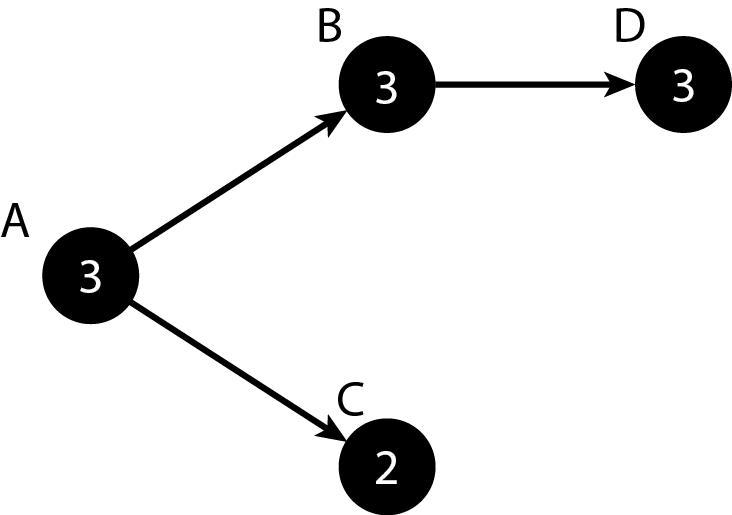
\includegraphics[scale=0.4]{./figures/delay_factor.png}}
\caption{Delay factors are given for courses A, B, C, and D.} 
\label{fig:delay_factor_example}
\end{figure}

A course's blocking factor is defined as the number of courses that are blocked from being taken if the given courses is not passed. This is essentially the connectivity of the course. If there is a path from \(i\) to \(j\) then \(n_{ij}\) is 1 and 0 otherwise. Then, the blocking factor of course i would be given by

\begin{equation}
  V_{i} = \sum_{j} n_{ij}
\end{equation}

An example of blocking factors can be seen in Figure \ref{fig:blocking_factor_example}. Here, course A has a blocking factor of three because it is connected (blocks) three other courses: B, C and D. Coure B blocks one course, D and courses C and D have a blocking factor of zero because no coures succeed them.

\begin{figure}[h!]
\centerline{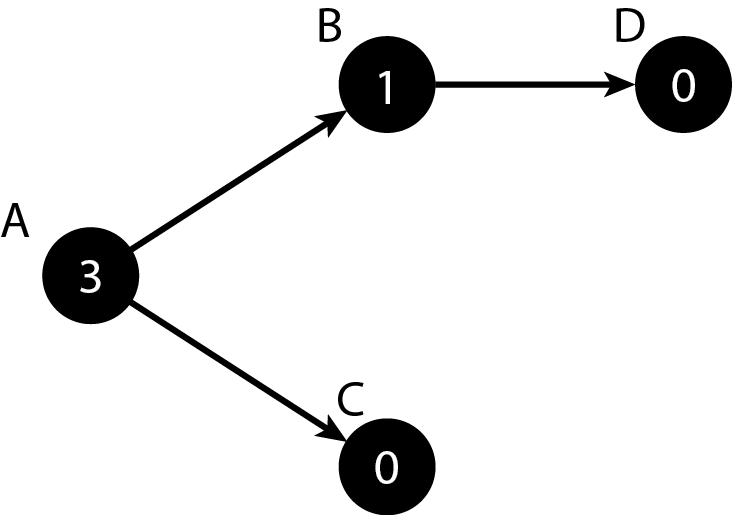
\includegraphics[scale=0.4]{./figures/blocking_factor.png}}
\caption{Blocking Factors are given for courses A, B, C, and D.} 
\label{fig:blocking_factor_example}
\end{figure}

Given a courses delay factor path, \(L_i\), and blocking factor, \(V_i\), then it's cruciality, \(C_i\) is simply given by the sum of the two:

\begin{equation}
  C_{i} = V_{i} + L_{i}
\end{equation}

A curriculum's complexity, \(S\) is then given by the sum over all course crucialities:

\begin{equation}
  S = \sum_{i}^n C_{i}
\end{equation}

While it is far from the only factor for student success, it is intuitive to see that a curriculum's structural complexity can impact the time in which it takes students to move through a program. Students that fail a course with a high blocking factor will be unable to take needed courses the following semester potentially delaying them and curricula with high blocking factors present many opportunities for being delayed. Curricula with long paths, and therefore high delay factors, can also delay students and even impose minimum term completion limits. For example, a curricula with a long path of eight requires at least four years to complete and if a course on that path is failed, the student will be delayed at least one semester.

\section{Correlating Complexity with Completion Rates}

One of the motivations for the development of the curriculum flow simulation is to show that there is a correlation between structural complexity and the rates at which students complete the curricula. As a start, several tests were carried out over extreamly simple curricula seen in \ref{fig:simple}. These curricula, consisting of two terms with two courses each make up common patterns that can be found in actual curricua and span a range of complexity values making them good candiates to observe how structure affects the way students flow through curricula.

\begin{figure}
\centering
\begin{subfigure}[h!]{.3\linewidth}
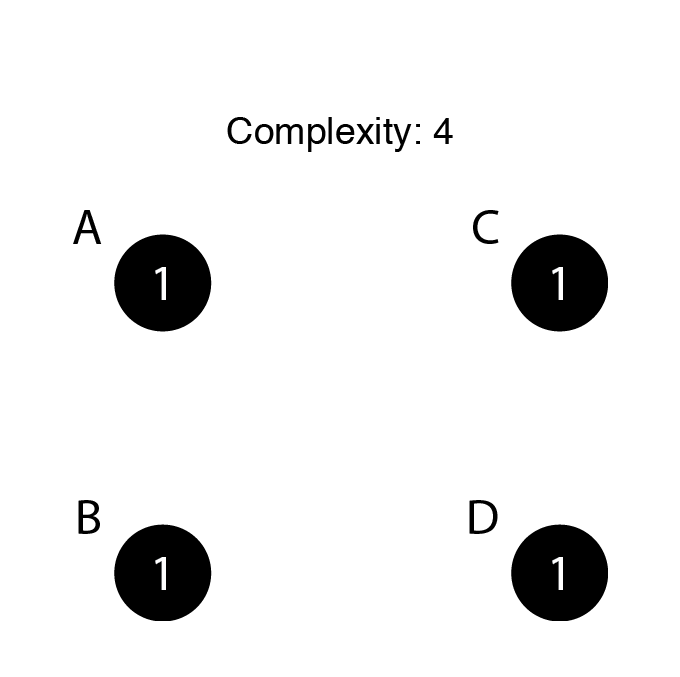
\includegraphics[width=\linewidth]{./figures/Simple4.png}
\caption{Curriculum One}\label{fig:simple4}
\end{subfigure}
\begin{subfigure}[h!]{.3\linewidth}
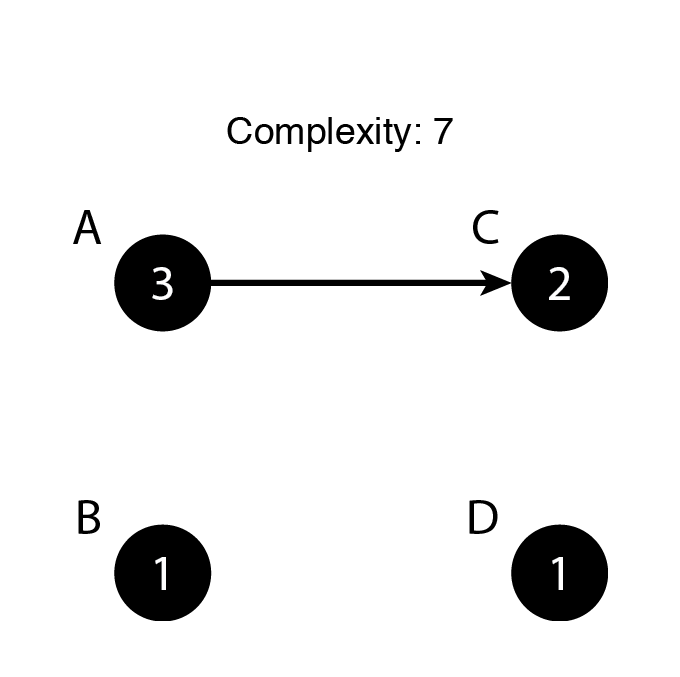
\includegraphics[width=\linewidth]{./figures/Simple7.png}
\caption{Curriculum Two}\label{fig:simple7}
\end{subfigure}
\begin{subfigure}[h!]{.3\linewidth}
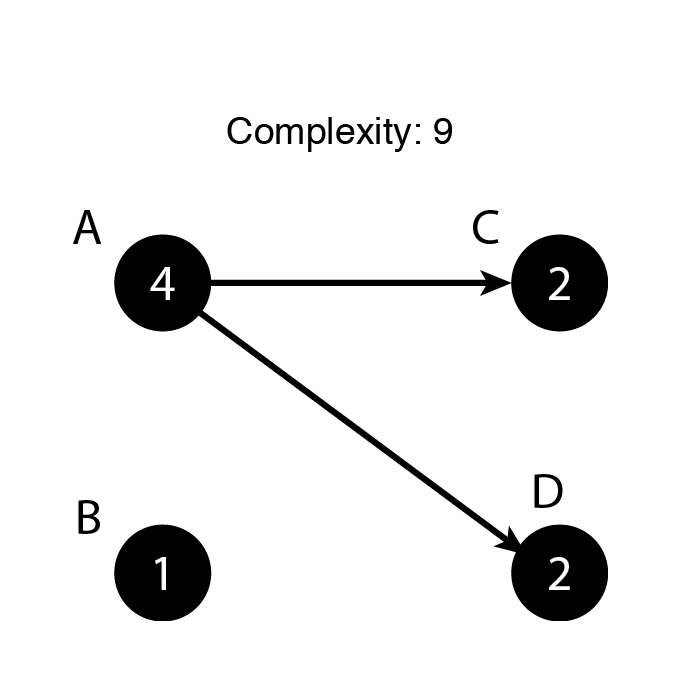
\includegraphics[width=\linewidth]{./figures/Simple9-1.png}
\caption{Curriculum Three}\label{fig:simple91}
\end{subfigure}

\begin{subfigure}[h!]{.3\linewidth}
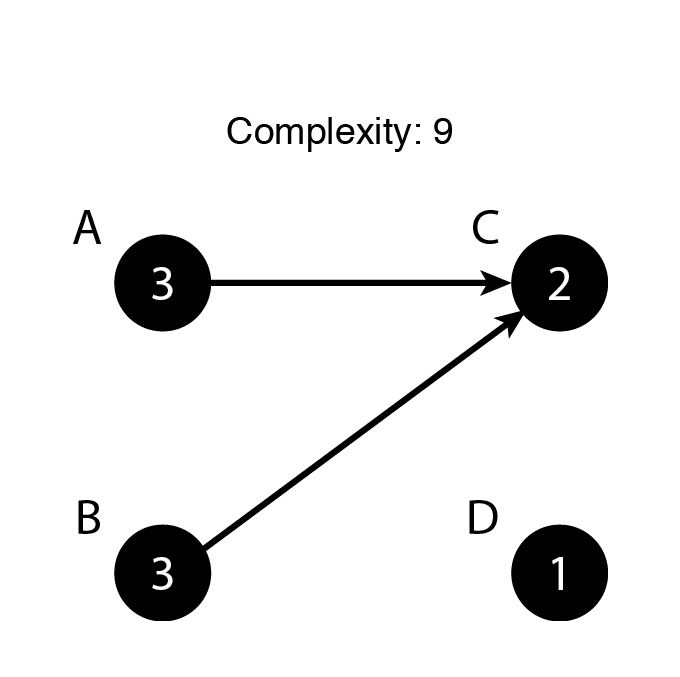
\includegraphics[width=\linewidth]{./figures/Simple9-2.png}
\caption{Curriculum Four}\label{fig:simple92}
\end{subfigure}
\begin{subfigure}[h!]{.3\linewidth}
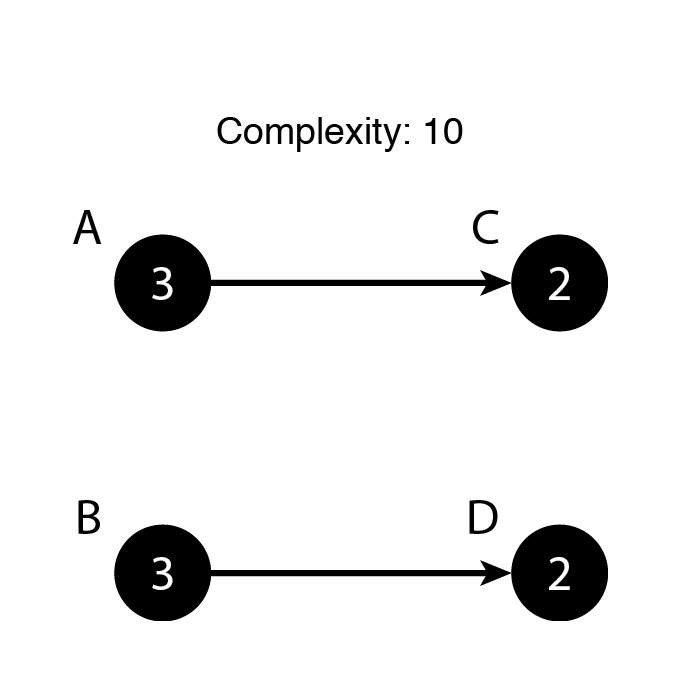
\includegraphics[width=\linewidth]{./figures/Simple10.png}
\caption{Curriculum Five}\label{fig:simple10}
\end{subfigure}

\caption{Basic Curricula}
\label{fig:simple}
\end{figure}

Each simulation carried out over the five curricula using the following configuration. The simulation's default performance module is used meaning that a student is determined to either pass or fail based on the corse's passrate. Every course has a passrate of 50\%, therefore each student has a one in two chance of passing the course. The simulation's duration is four semesters, and a student is allowed to take up to nine credit hours a semester with each course counting for three. Each curriculum is simulated one hundred times with one hundred students each and the results from each are then averaged. The results can be seen in Table \ref{tab:simpleResults}.

\begin{table}[!h]
  \tiny
  \caption{}
  \begin{subtable}{0.45\linewidth}
    \centering
      \caption{Curriculum One}
      \label{tab:simple4}
      \begin{tabular}{l*{4}{c}}
        Course  & Term 1 & Term 2 & Term 3 & Term 4 \\
        \hline
        A       & 49.62 & 75.2  & 87.33 & 93.73 \\
        B       & 50.64 & 75.48 & 87.64 & 93.97 \\
        C       & 49.98 & 75.62 & 87.98 & 94.14 \\
        D       & 0.0 & 44.1 & 71.89 & 85.77 \\
        \hline
        Completion \\ Rate & 0.0 & 20.72 & 49.5 & 71.63
      \end{tabular}
  \end{subtable}\hfill
  \begin{subtable}{0.45\linewidth}
    \centering
      \caption{Curriculum Two}
      \label{tab:simple7}
      \begin{tabular}{l*{4}{c}}
        Course  & Term 1 & Term 2 & Term 3 & Term 4 \\
        \hline
        A       & 51.19 & 75.31 & 87.23 & 93.48 \\
        B       & 49.94 & 74.71 & 87.31 & 93.45 \\
        C       & 0.0   & 25.5  & 51.27 & 69.39 \\
        D       & 49.3  & 75.2  & 87.31 & 93.59 \\
        \hline
        Completion \\ Rate & 0.0 & 14.35 & 39.21 & 60.41 \\
      \end{tabular}
  \end{subtable}

  \vspace*{1cm}
  \begin{subtable}{0.45\linewidth}
    \centering
      \caption{Curriculum Three}
      \label{tab:simple91}
      \begin{tabular}{l*{4}{c}}
        Course  & Term 1 & Term 2 & Term 3 & Term 4 \\
        \hline
        A & 49.96 & 74.78 & 87.43 & 93.38 \\
        B & 49.68 & 74.57 & 87.28 & 93.95 \\
        C & 0.0   & 25.59 & 50.51 & 69.2  \\
        D & 0.0   & 24.61 & 49.64 & 68.83 \\
        \hline
        Completion \\ Rate & 0.0   & 8.88  & 30.01 & 52.57 \\
      \end{tabular}
  \end{subtable} 
  \hfill
  \begin{subtable}{0.45\linewidth}
    \centering
      \caption{Curriculum Four}
      \label{tab:simple92}
      \begin{tabular}{l*{4}{c}}
        Course  & Term 1 & Term 2 & Term 3 & Term 4 \\
        \hline
        A & 49.98 & 75.12 & 87.93 & 93.92 \\
        B & 49.76 & 75.44 & 87.37 & 93.73 \\
        C & 0.0   & 12.35 & 34.7  & 55.21 \\
        D & 49.98 & 75.4  & 87.79 & 94.33 \\
        \hline
        Completion \\ Rate & 0.0   & 9.31  & 30.44 & 52.3  \\
      \end{tabular}
  \end{subtable}

  \vspace*{1cm}
  \begin{subtable}{0.45\linewidth}
    \centering
      \caption{Curriculum Five}
      \label{tab:simple10}
      \begin{tabular}{l*{4}{c}}
        Course  & Term 1 & Term 2 & Term 3 & Term 4 \\
        \hline
        A & 49.9  & 74.99 & 87.75 & 93.6  \\
        B & 49.93 & 75.1  & 88.0  & 94.05 \\
        C & 0.0   & 25.21 & 50.07 & 68.75 \\
        D & 0.0   & 24.61 & 49.47 & 68.61 \\
        \hline
        Completion \\ Rate & 0.0   & 6.07  & 24.5  & 46.93 \\
      \end{tabular}
  \end{subtable} 
  \label{tab:simpleResults}
\end{table}

These tables show the percentage of students that have passed each course at the end of each semester. For example in Table \ref{tab:simple4}, 75.2\% of students had passed Course A after the second semester. The row at the bottom then shows the percetage of students that had completed all courses at the end of each term. As expected, the least complex curricula resulted in the hight completion rates after four terms with the completion rates dropping as complexity increased. Its also important to note that the two curricula with the same complexity had very similar completion rates despite their structures being slightly different.

\end{document}